\chapter{Podstawowe pojęcia}
\label{c2}

W niniejszym rozdziale zostaną zawarte podstawowe pojęcia i mechanizmy używane przez aplikację App Inventor. Ideą jest tutaj przybliżenie ważnych terminów informatycznych.

\section{Główne komponenty}
\label{c22}

App Inventor celowo ułatwia programowanie poprzez wizualizację tworzonych komponentów i intuicyjny interfejs. App Inventor składa się z 3 głównych komponentów, jakimi są:
\begin{itemize}
\item App Inventor Designer
\item App Inventor Blocks Editor
\item Android Device Emulator
\end{itemize}

\subsection{App Inventor Designer}
\label{c221}

Jednym z głównych widoków których można używać jest widok Designera. Projektowanie interfejsu użytkownika polega na przeciąganiu komponentów z dostępnej palety, wliczając w to także niewidoczne komponenty, takie jak sensory. W tym widoku można również zmieniać właściwości obiektów, które zostały stworzone. Między innymi istnieje możliwość zmiany położenia, wielkości, układu (pionowy, poziomy).

Designer jest zaprojektowany jako zwykła aplikacja internetowa. Tak więc uruchamia się go, jak zwykłą stronę internetową wpisując jej adres www.

\begin{figure}[th] 
\centering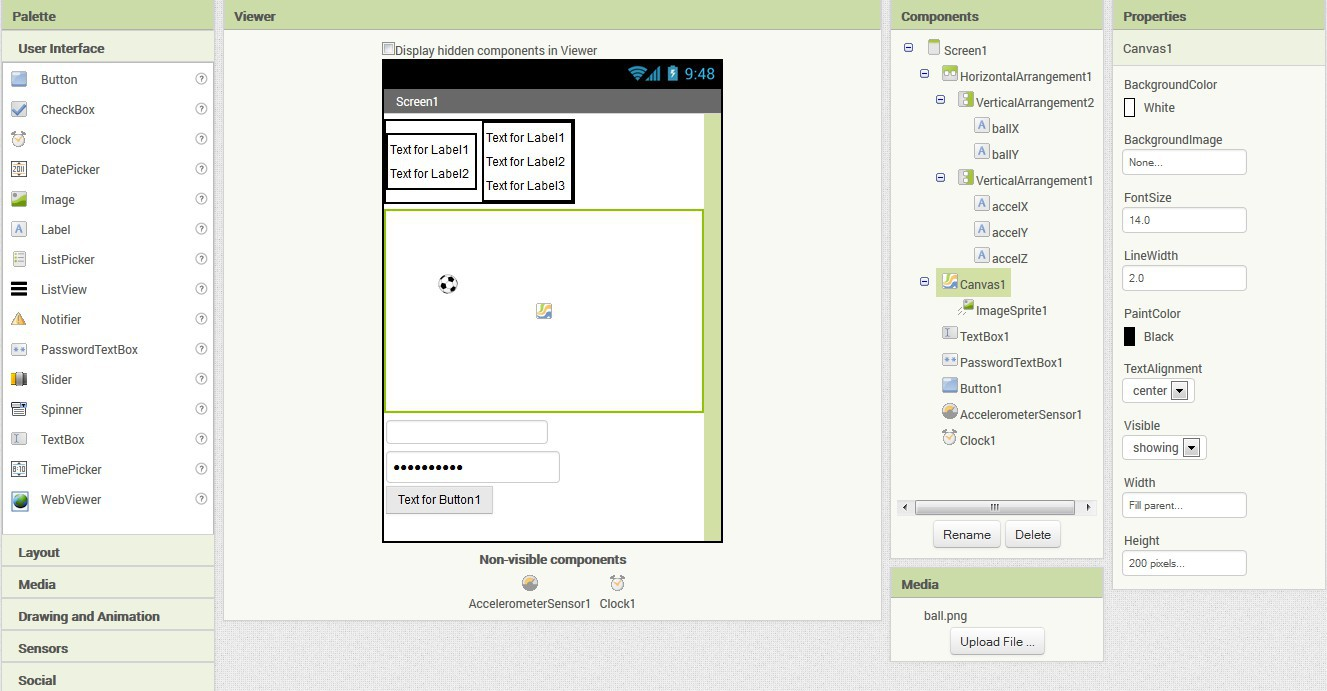
\includegraphics[width=10cm]{figures/designer}
\caption{App Inventor Designer}
\end{figure}

\subsection{App Inventor Blocks Editor}
\label{c222}

Drugim widokiem jest Blocks Editor. Zachowanie aplikacji zostaje tutaj zaprogramowane poprzez połączenie odpowiednich bloków. Istnieje możliwość korzystania z bardziej generalnych komponentów, a także z bardziej specyficznych. Dla każdego komponentu, który został stworzony w interfejsie graficznym (Designerze) są dostępne bloki mówiące, co tak naprawdę jest możliwe do zrobienia. Wygląda to w ten sposób, że komponenty są przciągane z dostępnej palety metodą "przeciągnij i upuść", a następnie łączone jak puzzle.

Ta część aplikacji normalnie reprezentowana jest przez kod napisany przez programistę. Zatem napisanie zachowania aplikacji odbywa się poprzez łączenie puzzli, bez wymogu znajomości języka Java.

\begin{figure}[th] 
\centering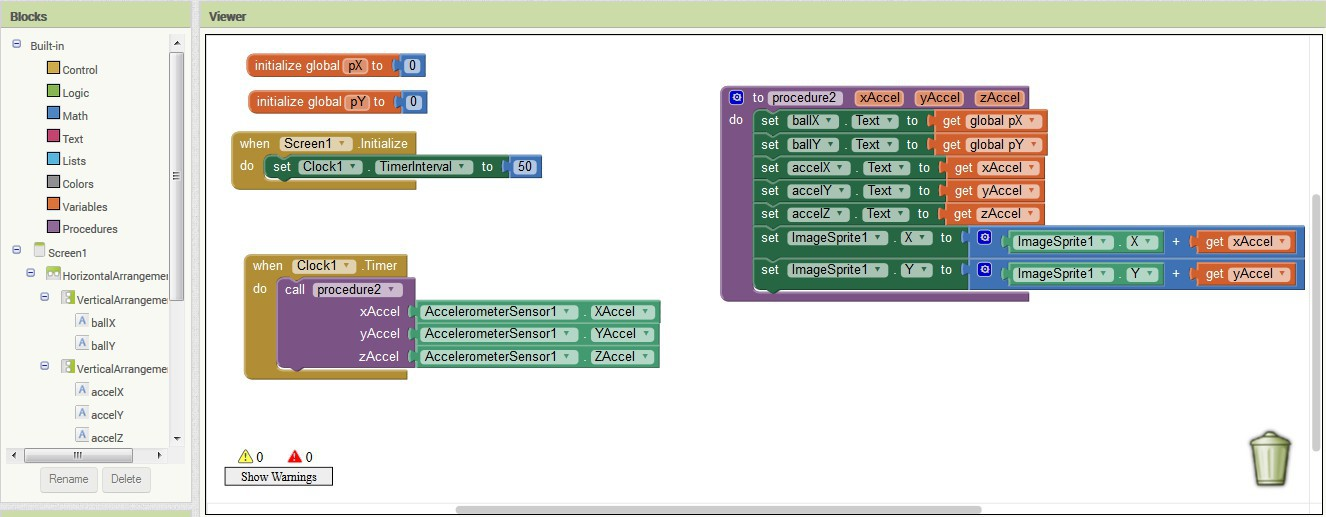
\includegraphics[width=10cm]{figures/editor}
\caption{App Inventor Blocks Editor}
\end{figure}

\subsection{Android Device Emulator}
\label{c223}

Android Device Emulator jest to emulator telefonu lub tabletu. Przedstawia on wirtualną wersję smartphonu, w której znajdują się obsługa dotyku ekranu, przyciski systemowe oraz typowe funkcje.

Wprowadzone zmiany, natychmiast reflektują na działanie aplikacji. Nie ma potrzeby jakiejkolwiek kompilacji i uruchamiania aplikacji od nowa. Jeżeli aplikacja zostanie uruchomiana, kompilacja zmienionych fragmentów oraz zainstalowanie ich na emulatorze dzieje się w czasie rzeczywistym. Jest to bardzo wygodna opcja budowania aplikacji i testowania jej. Zmiany, które zrobimy, są od razu widoczne na ekranie.

\begin{figure}[th] 
\centering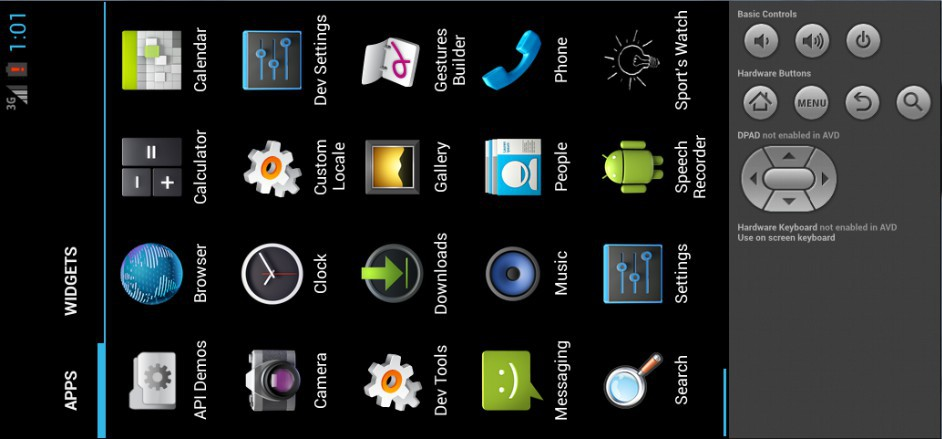
\includegraphics[width=10cm]{figures/emulator}
\caption{Android Device Emulator}
\end{figure}

\section{System operacyjny Android}

Android jest systemem operacyjnym stworzonym na urządzenia mobilne. Bazuje on na systemie Linux i aktualnie rozwijany jest przez firmę Google. Android stworzony jest głównie do urządzeń posiadająych ekran dotykowy, są to między innymi tablety i smartphony. System reaguje na dotyk w różnych postaciach. Odpowiada to takim gestom jak, pukanie, szczypanie, przesuwanie palcem (\english{Swipe}). Pomimo tego że system został głównie zaprojektowany dla ekranów dotykowych znalazł także zastosowanie w grach na konsolę, kamerach i innej elektronice.

Anroid jest jendym z najbardziej popularnych systemów operacyjnych na platformę mobilną. W 2013 roku sprzedano ich więcej niż łączna suma pozostałych znanych marek, za którymi kryją się Windows, iOS, Mac OS.\cite{android:1}\cite{android:3}\cite{android:3}\cite{android:4} W lipcu 2013 roku market Google Play posiadał ponad 1 milion opublikowanych aplikacji oraz ponad 50 miliardów pobrań.\cite{android:5} Na przełomie kwietnia i maja 2013 roku została przeprowadzona ankieta wśród programistów. Okazało się, że 71\% programistów, którzy tworzą aplikacje mobilne, tworzą je na system Android.\cite{android:6}

Android okazał się popularny wśród firm, które wymagają gotowych, tanich rozwiązań oraz system operacyjny, który można dostosować do własnych preferencji.\cite{android:7} Otwarta natura Androida zachęciła dużą część programistów oraz entuzjastów do użycia ogólno dostępnego kodu jako podstawa do tworzonych projektów.\cite{android:8}

\subsection{Historia}

Firma Android została założona w Palo Alto, w Kalifornii w październiku 2003 roku w celu opracowania inteligentnych urządzeń mobilnych, które są bardziej świadome położenia i preferencji niż sam właściciel telefonu.\cite{android:9} Pierwotnym założeniem firmy było opracowanie zaawansowanego systemu operacyjnego dla aparatów cyfrowych, jednak zdano sobie sprawę, że liczba urządzeń tego typu na rynku nie była zbyt duża. Wówczas dopiero celem stały się systemy operacyjne smartphonów. Głównymi rywalami w tamtych czasach były sysytemy operacyjne: Symbian i Windows Mobile.\cite{android:10} Mimo poprzednich osiągnięć założycieli i pierwszych pracowników firma Android działała potajemnie, ujawniając tylko, że pracuje nad oprogramowaniem dla telefonów komórkowych.\cite{android:9}

W sierpniu 2005 roku firma Google przejęła firmę Android. Kluczowi pracownicy, wliczając w to niektórych założycieli, pozostali w firmie po przejęciu.\cite{android:9} W tym czasie nie wiele wiedziano o firmie Android ale zakładano, że Google zamierza wejść na rynek telefonów komórkowych.\cite{android:9} Zespół pracujący nad systemem operacyjnym kierowany przez jednego z pierwotnych założycieli opracował mobilną platformę opartą o jąrdo Linuksa. Google zaczął reklamować platformę, kierując reklamę w stronę producentów telefonów komórkowych, obiecując zapewnienie elastycznego systemu operacyjnego, który będzie można łatwo aktualizować. Po zakończeniu akcji marketingowej Google zdobył szereg partnerów, wyrażających chęć współpracy.\cite{android:11}\cite{android:12}\cite{android:13}

Spekulacje o zamiarze wejścia Google na rynek urządzeń mobilnych były kontynuowane przez grudzień 2006 roku.\cite{android:14} Prototyp o nazwie kodowej \emph{Sooner} był podobny do modelu BlackBerry, tyle że był stworzony bez ekranu dotykowego i klawiatury QWERTY. Dopiero później został ponownie zaprojektowany aby obsługiwać ekran dotykowy i konkurować z innymi urządzeniami takimi jak LG Prada, Apple iPhone.\cite{android:15}\cite{android:16}

W październiku 2007 roku Open Handset Alliance - konsorcjum firm technologicznych w tym Google, producenci urządzeń takich jak HTC, Samsung, Sony, operatorów bezprzewodowych m.in. T-Mobile oraz producenci mikroukładów zaprezentowało się, w celu stworzenia otwartych standardów dla telefonów komórkowych.\cite{android:17} Tego dnia Android pokazał ukazał swój pierwszy produkt, mobilna platforma oparta o jądro Linuksa w wersji 2.6.25.\cite{android:17}\cite{android:18} Pierwszy dostępny komercyjnie smartfon z systemem Android był HTC Dream, wydany w październiku 2008 roku.\cite{android:19}

W 2010 roku Google rozpoczął produkować serię urządzeń pod nazwą Nexus - linia smartphonów i tabletów z systemem operacyjnym Android. Pierwszy Nexus One został wyprodukowany przez partnera Google firmę HTC.\cite{android:20} Google wprowadziło na rynek nowe urządzenia z serii Nexus, jako ich sztandarowe produkty, demonstrując najnowsze funkcje systemu Android.

Od 2008 roku Android wprowadzał wiele aktualizacji, które stopniowo doskonalały pierwotny system, dodając nowe funkcje i poprawiając błędy w poprzednich wersjach. Każda główna wersja systemu została nazwana w konwencji alfabetycznej po nazwie deseru lub innej słodkości. Przykładami są tutaj: wersja 1.5 Cupcake, następnie wersja 1.6 Donut. Ostatnia wersja 4.4.4 KitKat pojawiła się tylko jako aktualizacja zabezpieczeń, została wydana w czerwcu 2014 roku, krótko po wydaniu wersji poprzedniej 4.4.3.\cite{android:21}\cite{android:22}\cite{android:23}

\subsection{Interfejs}

Domyślny interfejs użytkownika bazuje na bezpośredniej manipulacji\cite{android:24} dotykiem, który odpowiada za manipulację obeiktów znajdujących się na ekranie oraz wirtualnej klawiatury. \cite{android:24} Opowiedź na dany ruch użytkownika jest natychmiastowa, zapewniając płynność, często z wykorzystaniem funkcji wibracji urządzenia. Wenętrzny sprzęt zawarty w telefonie taki jak akcelerometr, żyroskop, czujnik optyczny, jest wykorzystywany przez niektóre aplikacje aby zapewnić odpowiedź na niektóre ruchy użytkownika.\cite{android:25} Przyładem takiej aplikacji jest regulowanie ekranu z poziomego na pionowy, w zależności od tego jak urządzenie jest zorientowane. Kolejnym przykładem są gry pozwalające sterowanie pojazdem poprzez obrót urządzenia, symulując prawdziwą kierownicę.\cite{android:26}

System android uruchamia się do ekranu startowego, który jest jest głównym punktem nawigacji i informacji o urządzeniu. Zachowanie to jest podobne do zachowania znanego z komputerów stacjonarnych. Ekran startowy w Androidzie zazwyczaj składa się ikon, które uruchamiają powiązane aplikacje, widżetów, które odświeżają się automatycznie i wyświetlają aktualne informacje. Przykładami są np. widżety pokazujące pogodę, powiadomienia skrzynki pocztowej, dzienne wiadomości.\cite{android:27} Ekran startowy w większości przypadków jest stworzony z kilku stron, które użytkownik może przesuwać. Ponad to ekran ten jest mocno konfigurowalny, pozwalając użytkownikowi dostosować wygląd urządzenia do jego gustu.\cite{android:28} Apliakcje osób trzecich dostępne w markecie Google Play, a także innych marketach mogą zdecydowanie zmienić interfejs użytkownika, a nawet naśladować wygląd innych systemów operacyjnych takich jak Windows Phone.\cite{android:29} Większość producentów i niektórzy operatorzy komórkowi mogą dostosować wygląd swoich urządzeń aby różnić się od konkurencji. \cite{android:30}

W górnej części ekranu znajduje się pasek stanu, przedstawiający informacje na temat urządzenia i jego połączenia. Pasek ten można przeciągnąć w dół, aby odsłonić ekran powiadomień, gdzie wyświetlane są ważne informacje i aktualizacje, takie jak e-mail, nieodebrane połączenie. Rozwinięty pasek stanu przedstawiony jest na rysunku poniżej:

\begin{figure}[H] 
\centering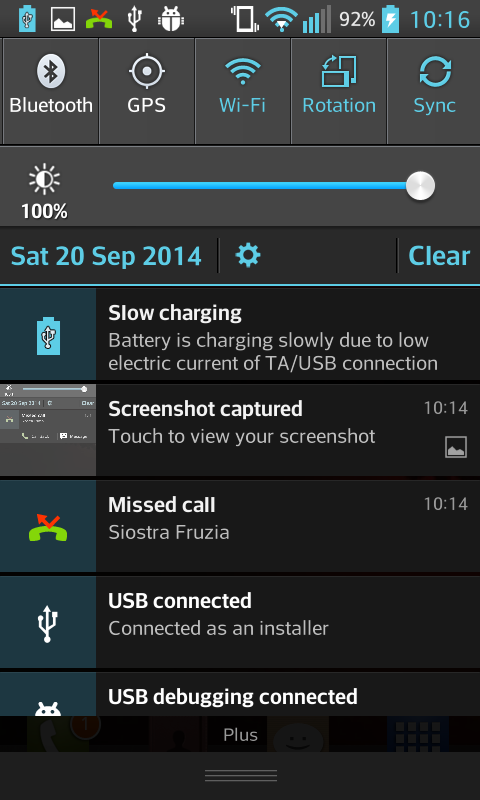
\includegraphics[width=6cm]{figures/android/statusbar}
\caption{Pasek stanu z różnymi powiadomieniami}
\end{figure}

Powiadomienia te są widoczne, aż użytkownik kliknie na nie uruchamiając powiązaną z nimi aplikację, lub odrzuci je przesuwając palcem w lewo lub w prawo na danym powiadomieniu. W wersji systemu 4.1 Android wprowadził rozszerzone powiadomienia. W pasku stanu mogą być wyświetlane dodatkowe funkcje. Przykładem jest odtwarzacz muzyki umożliwiający sterowanie odtwarzaniem lub powiadomienie o nieodebranym połączeniu. Powiadomienie to zawiera przyciski umożliwiające oddzwonienie lub wysłanie wiadomości zwrotnej.\cite{android:31}

\subsection{Aplikacje}

System Android posiada bardzo duży wybór wśród aplikacji, które użytkownik może zainstalować. Aplikacje te mogą zostać zainstalowane za pośrednictwem marketu Google Play, Amazon Appstore lub zainstalowanie pliku \emph{.apk} aplikacji ze strony osób trzecich.\cite{android:32} Market Google Play pozwala użytkownikom na przeglądanie, pobieranie i aktualizację aplikacji opublikowanych przez Google oraz innych programistów. Aby pobierać aplikacje z witryny, użytkownik musi posiadać aplikację Google Play na urządzeniu mobilnym. Jest to aplikacja instalowana fabrycznie. Google Play filtruje listę dostępnych aplikacji do tych, które są kompatybilne z urządzeniem. Programisci przy publikowaniu aplikacji mają możliwość ograniczenia swoich aplikacji do poszczególnych operatorów komórkowych lub krajów z powodów biznesowych.\cite{android:33}

Od lipca 2013 roku istnieje ponad milion aplikacji dostępnych dla systemu Android w markecie Google Play.\cite{android:34} Od maja do lipca 2013 roku, zatem w ciągu 3 miesięcy liczba instalacji wzrosła o 2 miliardy osiągając 50 miliardów.\cite{android:34}\cite{android:35}

Aplikacje tworzone są głównie za pomocą języka Java przy użyciu Android SDK. Są to biblioteki programistyczne i zostały dokładniej przedstawione w dalszej części pracy. Inną możliwością tworzenia aplikacji jest App Inventor. Narzędzie dla początkujących programistów, umożliwiające programowanie wizualne.

\subsection{Zarządzanie pamięcią}

Urządznie z systemem Android zazwyczaj zasilane są z baterii. Android został zaprojektowany, aby zarządzać pamięcią RAM, tak aby utrzymać zurzycie energii na najniższym poziomie. Jest to przeciwieństwo do standardowych systemów operacyjnych instalowanych na komputerach, które zakładają, że są już podłączone do nieograniczonej sieci elektrycznej. Kiedy uruchomiona aplikacja nie jest w użyciu, system automatycznie może zawiesić ją w pamięci. Aplikacja nadal jest technicznie uruchomiona, ale nie zużywa żadnych zasobów, pozostając bezczynnie w tle, dopóki znowu będzie potrzebna. Ma to podwójną korzyść, zwiększenie ogólnej reaktywności urządzeń, ponieważ aplikacje nie muszą być zamykane i uruchamiane ponownie od zera, a także zapewnienie, że aplikacje działające w tle nie zużywają niepotrzebnie energii.\cite{android:36}\cite{android:37}

\begin{figure}[H] 
\centering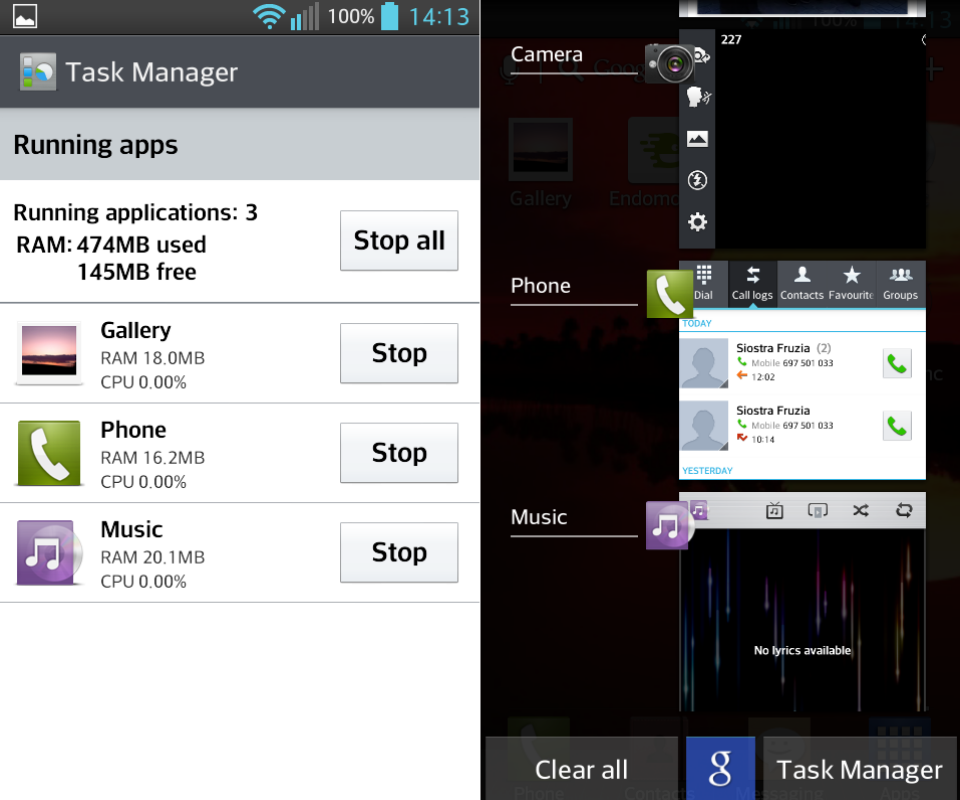
\includegraphics[width=8cm]{figures/android/memoryManagment}
\caption{Menadżer urządzeń oraz pogląd uruchomionych aplikacji}
\end{figure}

Na powyższym rysunku po lewej stronie został pokazany menadżer urządzeń. Użytkownik może odczytać jakie jest zużycie procesora uruchomionych aplikacji, które działają w tle. Istnieje także możliwość ich zatrzymania i usunięcia z pamięci RAM. Po prawej stronie użytkownik ma możliwość szybkiego poglądu ruchomionych aplikacji oraz zamknięcia ich.

\subsection{Wykorzystanie platformy}

Poniższa tabela prezentuje strukturę wersji Androida. Bazuje ona na  urządzeniach korzystających z Play Store we wrześniu 2014 roku. Dane zostąły zebrane podczas jednego tygodnia.\cite{android:38}

\begin{figure}[H] 
\centering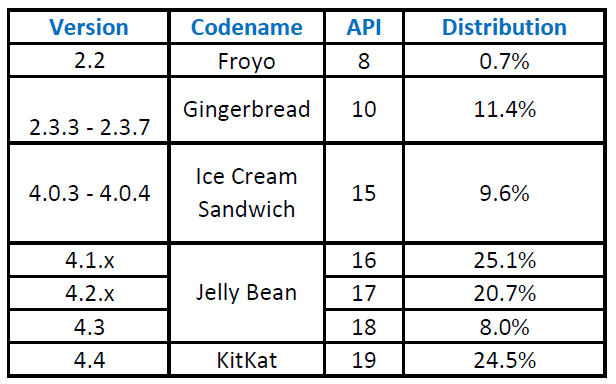
\includegraphics[width=8cm]{figures/android/distributionChart}
\caption{Tabela przedstawiająca rozkład wersji systemu}
\end{figure}


Należy pamiętać, że powyższa tabela nie obejmuje urządzeń Android, które nie korzystały z Google Play.


\section{Pozostałe istotne komponenty}

W niniejszym rozdziale zawarto pozostałe komponenty, które zostały użyte podczas pisania pracy. Związane są one zarówno z App Inventorem, jak i z aplikacjami napisanymi w Javie.

\subsection{Android SDK}

Adnroid SDK to zestaw narzędzi programistycznych oferowanych dla programistów zamierzających tworzyć aplikacje na platformę Android. Jest on modularny, poprzez SDK Managera możemy zainstalować tylko te komponenty, które nas interesują.
 
\subsection{SDK Tools}

Android SDK dzieli się na dwie części: SDK Tools oraz Platform Tools. Najważniejsze narzędzia wchodzące w skład pierwszej części to:
\begin{itemize}
\item AVD Manager - odpowiedzialny za zarządzanie wirtualnymi urządzeniami z systemem operacyjnym Android. Jest to najłatwiejsza i najwygodniejsza opcja stworzenia nowego wirtualnego urządzenia i odpowiedniego sparametryzowania go.
\item SDK Manager - wspomniany wyżej, odpowiedzialny za instalację modułów, które nas interesują.
\item Emulator - emualtor systemu android, stworzony przez AVD Managera.
\item Dalvik Debug Monitor (DDMS) \label{ddms}- jest to narzędzie pomocne w debugowaniu aplikacji. Dostarcza on takich funkcji jak przekierowanie portów, przechwyt obrazu na urządzeniu, informacje o wątkach, stosie, a także o metodach, które są uruchomione jeżeli włączymy ich profilowanie.
\end{itemize}

\subsection{Platform Tools}

\begin{itemize}
\item Android Debug Bridge \label{adb}- narzędzie pozwalające na komunikację z podłączonym urządzeniem. Jest także używany do instalacji i uruchamiania aplikacji. Składa się z 2 części, klienta i serwera, które komunikują się ze sobą.
\end{itemize}

\subsection{Apktool}

Jest to narzędzie do tak zwanej inżynierii odwrotnej (\english{Reverse engineering}). Umożliwia ono dekodowanie programu do prawie oryginalnej formy. Następnie, po dokonaniu pewnych modyfikacji, umożliwia ono zbudowanie aplikacji z powrotem do wyjściowej formy.\cite{doc:apktool}

\subsection{Keystore}

Jest to repozytorium przechowujące certyfikaty bezpieczeństwa. Do zarządzania certyfikatami istnieje narzędzie o nazwie keytool. Umożliwia ono użytkownikom zarządzanie prywatnymi/publicznymi kluczami, certyfikatami jak i podpisem elektornicznym.\cite{doc:keytool}

\subsection{Jarsigner}

System Android wymaga, aby aplikacje na nim instalowane były cyfrowo podpisane. Dzięki temu system może zweryfikować autora aplikacji. Podpisywanie aplikacji dzielimy na 2 sposoby: tryb debugowania (\english{Debug mode})oraz tryb wydania (\english{Release mode}). Przy korzystaniu ze zintegrowanego środowiska programistycznego zwykle aplikacja zostaje cyfrowo podpisana automatycznie, podczas instalacji jej na telefonie. Jarsigner umożliwia popisanie aplikacji manualnie, korzystając z linii poleceń.

\subsection{Zużycie procesora}

Czas pracy procesora jest to czas, w którym procesor (\english{CPU}) został użyty to przetwarzania zadanych instrukcji, w przeciwieństwie do oczekiwania na wejście/wyjście lub przejścia w stan oczekiwania (\english{Idle mode}). Zużycie procesora natomiast mierzone jest w procentach jako całkowita wydajność procesora. Główne zastosowanie to określenie ogólnej zajętości systemu. Wysokie zużycie procesora oznacza zbyt małą moc procesora, lub zbyt wygórowane oczekiwania użytkownika.


\section{Ważne koncepcje i pojęcia dotyczące App Inventora}

Istnieje kilka pojęć, które są warte uwagi. Zostały one zawarte w tym rozdziale.

\subsection{Publikacja aplikacji na Google Play}

Aplikacje zbudowane za pomocą App Inventora mogą zostać przesłane do marketu Google Play. Każda aplikacja, która ma zostać opublikowana musi posiadać wersję kodu (\english{VersionCode}) oraz nazwę wersji (\english{VersionName}). Te parametry można ustawić we właściwościach głównego komponentu\cite{doc:concepts}. Wersja kodu jest to całkowita wartość, która nie jest widoczna dla użytkowników w Google Play. Potrzebna jest do sprawdzenia, czy aplikacja została aktualizowana lub dezaktualizowana do poprzedniej wersji. Nazwa wersji może być dowolna, jednak wg konwencji powinna to być liczba zmiennoprzecinkowa. Domyślnie posiada wartość 1.0. Jest ona zwiększana o 0.1 lub 1 dla małej i dużej zmiany.

Skończony projekt możemy wyeksportować do pliku .apk, który jest automatycznie cyfrowo podpisany kluczem prywatnym powiązanym z naszym kontem. Kiedy tworzymy nową wersję, ten sam klucz jest używany do podpisu. Kiedy urządzenie z system android posiada zainstalowaną aplikację, zapamiętuje on klucz który użyto do podpisu. Celem zainstalowania wyższej wersji należy zastosować do podpisu ten sam klucz. 

Repozytorium keystore, w którym znajduje się klucz, domyślnie jest stworzone na serwerze, więc nie potrzebujemy specjalnie go tworzyć. Istnieje również opcja eksportu i importu repozytorium. Jest ona przydatna przy przenoszeniu projektu na inny serwer.

\subsection{Paleta z dostępnymi komponentami}

\begin{itemize}

\item \textbf{User Interface} - w większości widoczne komponenty, które są związane z interfejsem użytkownika.
\begin{itemize}
\item Button - przycisk.
\item CheckBox - pole wyboru.
\item DatePicker - komponent dający możliwość wyboru daty.
\item Image - komponent umożliwiający wyświetlenie przesłanego zdjęcia.
\item Label - etykieta, na której zwykle wyświetlany jest kawałek tekstu.
\item ListPicker - komponent, który po kliknięciu wyświetla listę, z której użytkownik może wybrać wartość. Daje on także możliwość automatycznego osadzenia wyszukiwarki na liście.
\item ListView - komponent, który pozwala na osadzenie i wyświetlenie listy elementów.
\item Notifier - komponent wyświetlający powiadomienia, a także umożliwiający logowanie na 3 poziomach (Error, Warn, Info).
\item TextBox - komponent umożliwiający wpisywanie tekstu.
\item PasswordTextBox - taki sam komponent jak TextBox jednak wpisywany tekst nie jest widoczny dla użytkownika.
\item Slider - jest to pasek postępu, który dodatkowo umożliwia użytkownikowi przeciąganie.
\item Spinner - element wyświetlający pop-up z listą elementów do wyboru.
\item TimePicker - element pozwalający na wybór czasu.
\item WebViewer - komponenet umożliwiający umieszczenie dowolnej strony internetowej w aplikacji.
\end{itemize}

\item \textbf{Layout} - Komponenty odpowiedzialne za rozmieszczenie pozostałych komponentów. Są to kontenery, w które mogą zostać umieszczane inne widoczne komponenty.
\begin{itemize}
\item HorizontalArrangement - elementy umieszczone w tym kontenerze są układanej od lewej do prawej.
\item VerticalArrangement - odwrotne działanie do poprzedniego komponentu - elementy umieszcza się od góry do dołu.
\item TableArrangement - element umożliwiający ustawienie elementów postaci tabularnej
\end{itemize}


\item \textbf{Media} - Komponenty związane głównie z dźwiękiem oraz kamerą.
\begin{itemize}
\item Camcorder - komponent umożliwiający nagrywanie filmów. Istnieje możliwość nadania nazwy pliku zawierającego nagranie.
\item Camera - komponent umożliwiający robienie zdjęć i zapisywanie ich.
\item ImagePicker - komponent uruchamiający galerię zdjęć zawartą na telefonie i dający możliwość wyboru zdjęciu. Zdjęcie, po wybraniu, jest kopiowane na kartę SD (maksymalna ilość zdjęć to 10). Następnie możemy z danego zdjęcia skorzystać w aplikacji i je wyświetlić.
\item Player - komponent odtwarząjący muzykę, a także odpowiedzialny za wywołanie wibracji w telefonie.
\item Sound - komponent odtwarzający dźwięki, w porównaniu do poprzedniego, dźwięki powinny mieć krótki czas trwania, podczas gdy muzyka może być odtwarzana stosunkowo długo.
\item SoundRecorder - komponent nagrywający dźwięk.
\item SpeechRecognizer - komponent umożliwiający rozpoznanie mowy i stworzenie z niej tekstu.
\item TextToSpeech - komponent o odwrotnym działaniu do poprzedniego, zamieniający tekst na mowę. Wsparcie dla języków: czeskiego, hiszpańskiego, niemieckiego, francuskiego, duńskiego, włoskiego, polskiego, angielskiego.
\item VideoPlayer - komponent umożliwiający odtwarzanie filmu podczas działającej aplikacji. Pliki wideo muszą mieć poniżej 1MB, dodatkowo rozmiar całkowitej aplikacji wynosi maksymalnie 5MB.
\item YandexTranslate - komponent umożliwiający tłumaczenie tekstu pomiędzy językami. Korzysta on z serwisu o nazwie Yandex - https://translate.yandex.com. Dodatkowo urządzenie musi być podłączone do Internetu. 
\end{itemize}


\item \textbf{Drawing and Animation} Komponenty umożliwiające rysowanie oraz animacje.
\begin{itemize}
\item Canvas - płótno, na którym możemy rysować dwuwymiarowe obrazki (\english{Sprite}). Obrazki te mogą się na płótnie poruszać. Każda lokalizacja na płótnie jest specyfikowana za pomocą współrzędnych X,Y.
\item ImageSprite - obrazek, który możemy umieścić na płótnie i który może reagować na dotyk, przeciąganie.
\item Ball - jest to ImageSprite, który ma ustawiony obrazek jako koło o określanym kolorze.
\end{itemize}

\item \textbf{Sensors} Niektóre z sensorów, dostępnych na telefonie. Wszystkie z tych komponentów są niewidoczne.
\begin{itemize}
\item AccelerometerSenser - akcelerometr, komponent, który umożliwia wykrycie trzęsienia telefonem, podaje wartości, odpowiadające aktualnemu wychyleniu telefonu.
\item BarcodeScanner - komponent umożliwiający skanowanie kodów kreskowych, jednak musimy posiadać dodatkowo aplikację do tego zainstalowaną już na telefonie.
\item Clock - Zegar oraz czasomierz
\item LocationSensor - komponent dostarczający informacje o położeniu gdzie się znajdujemy, czyli szerokość i długość geograficzną. Informacje te mogą nie być od razu dostępne i musimy na nie poczekać.
\item NearField - komponent oferujący możliwośći NFC. Dotychczas komponent ten umożliwia czytanie i wysyłanie tagów tekstowych.
\item OrientationSensor - żyroskop - komponent dostarczający informację o urządzeniu w 3 wymiarach.
\end{itemize}

\item \textbf{Social} - komponenty związane z kontaktami, e-mailami i serwisami społecznościowymi.
\begin{itemize}
\item ContactPicker - przycisk, którego naciśnięcie powoduje wyświetlenie podlegających wyborowi kontaktów społecznościowych. Po dokonaniu wyboru użytkownik zyskuje dostęp do następujących danych: nazwa, e-maile, telefony, zdjęcie kontaktu.
\item EmailPicker - Textbox oferujący użytkownikowi pomoc, która polega na (automatycznym/ natychmiastowym) wyświetleniu listy adresów elektronicznych pasujących do aktualnie wpisywanego tekstu.
\item PhoneCall - komponent umożliwiający uruchomienie funkcji dzownienia do osoby, którą wcześniej ustawimy jako właściwość komponentu.
\item PhoneNumberPicker - przycisk o podobnym działaniu do komponentu ContactPicker.
\item Sharing - niewidoczny komponent, który umożliwia udostępnienie wiadomości lub pliku innym aplikacjom.
\item Texting - komponent odpowiedzialny za zarządzanie wiadomościami. Jeżeli aplikacja działa w tle, zdarzenie przyjścia wiadomości również będzie uruchomione. Nawet jeżeli aplikacja nie jest uruchomiona pojawi się powiadomienie o przyjściu wiadomości, po kliknięciu w nie uruchomi się aplikacja.
\item Twitter - komponent umożliwiający komunikację z serwisem internetowym Twitter. Jeżeli użytkownik zostanie pozytywnie zautentykowany i zautoryzowany, pojawia się wiele możliwości, m.in. szukanie tweetów, wysyłanie tweetów, wiadomości, obrazków.
\end{itemize}

\item \textbf{Storage} - komponenty odpowiedzialne za przechowywanie danych.
\begin{itemize}
\item File - niewidoczny komponent umożliwiający zapis i odczyt pliku. Domyślne ustawienia zapisują pliki do prywatnego katalogu App Inventora, jednak istnieje możliwość ustawienia innej ścieżki
\item FusiontablesControl - komponent, który komunikuje się z serwisem internetowym dostarczonym przez Google o nazwie Fusion Tables. Tabele te umożliwiają wizualizację, udostępnienie, zapis danych. Komponent ten daje możliwość dostępu do tych danych, a także jej edycji.
\item TinyDB - baza danych dla aplikacji. Jest to odpowiednik klasy Javy - SharedPreferences. Można sobie ją wyobrazić jako mapę - klucz/wartość.
\item TinyWebDB - niewidoczny komponent, komunikujący się z internetową bazą danych.
\end{itemize}

\item \textbf{Connectivity} - komponenty umożliwiające komunikację i uruchamianie innych apliakcji.
\begin{itemize}
\item ActivityStarter - komponent do uruchamiania zewnętrznych Activity. Przez Activity są rozumiane: inne aplikacje, kamera, wyszukiwarka internetowa, otwieranie strony internetowej, aplikacji mapy w zadanej lokalizacji. Tak naprawdę, możliwe jest wystartowanie dowolnej aplikacji, jednak trzeba znać nazwę pakietu (\english{package name}) oraz nazwę klasy (\english{class name}).
\item BluetoothClient - komponent blutetooth klienta.
\item BluetoothServer - komponent bluetooth serwera.
\item Web - komponenet umożliwiający wysyłanie żądań typu REST do serwera. Dostarcza od funkcje: GET, POST, PUT, DELETE.
\end{itemize}

\item \textbf{LEGO MINDSTORMS} - komponenty dostarczające kontrolę nad robotami poprzez bluetooth. W niniejszej pracy magisterskiej zostały pominięte, ze względu na brak powyższych robotów.
\end{itemize}

\subsection{Dostępne bloki}

\begin{itemize}

\item Control - bloki odpowiedzialne za przepływ informacji w aplikacji. Znajdują się tutaj instrukcje warunkowe if-else, pętle for, foreach, while, do-while. Inne bloki w tej sekcji są odpowiedzialne za otwieranie innych aplikacji lub zamykanie aktualnej.

\item Logic - bloki odpowiadające za logikę. Kiedy istnieje potrzeba stworzenia instrukcji warunkowej zazwyczaj korzysta się z tych bloków. Sprawdzają one, czy zmienne są takie same lub różne. Są tutaj też wartości true i false.

\item Math - bloki odpowiedzialne za wyrażenia matematyczne, min. takie jak dodawanie, odejmowanie, mnożenie, dzielenie. Ale są tu również funkcji pomocnicze, np. konwersja radianów do stopni lub odwrotnie, funkcje trygonometryczne, minimum dla zadanych argumentów, losowa wartość.

\item Test - bloki odpowiedzialne za zarządzanie tekstem. Jest tutaj większość funkcji znanej klasy String z Javy. Sprawdzenie czy zmienna jest pusta, ilość znaków, zamiana występnień danego elementu.

\item Lists - bloki tworzące listy oraz zarządzające nimi. Istnieje możliwość dodawania, usuwania, zamiany elementów na liście za pomocą oferowanych funkcji. Dodatkowe funkcji znajdujące się tutaj to funkcje konwertujące listę do formatu wiersza lub tabeli, który można następnie umieścić w pliku csv.

\item Colors - bloki z kolorami, które można przypisać stworzonym komponentom. Istnieje także możliwość zdefiniowania własnego koloru.

\item Variables - bloki odpowiedzialne za tworzenie zmiennych lokalnych i globalnych. Znajdują się tutaj też bloki inicjalizujące i odczytujące wartość zmiennych (\english{settery i gettery}).

\item Procedures - bloki tworzące procedury oraz funkcje zwracające wartość.

\end{itemize}

\subsection{Android - przechowywanie danych}

Urządzenie z systemem Android dostarcza szereg mechanizmów dotyczących przechowywania danych. Każdy z nich stosujemy do innych zadań.

\begin{itemize}
\item SharedPreferences - przechowuje pary klucz-wartość, czyli niewielkie ilości danych. Mechanizm wykorzystywany jest przede wszystkim do przechowywania ustawień aplikacji.\cite{tutorial:sqlite}
\item Baza danych SQLite – wykorzystywana do przechowywania dużej ilości uporządkowanych danych, które ze względu na swoją ilość wymagają wysokiej wydajności dostępu.\cite{tutorial:sqlite}
\item Pliki - w związku z wykorzystaniem bazy SQLite, która nie obsługuje przechowywania plików, dane binarne (zdjęcia, filmy, inne pliki) powinniśmy przechowywać w ich niezmiennej formie, na karcie lub pamięci wbudowanej w urządzenie.\cite{tutorial:sqlite}
\end{itemize}









